% Copyright 2004 by Till Tantau <tantau@users.sourceforge.net>.
%
% In principle, this file can be redistributed and/or modified under
% the terms of the GNU Public License, version 2.
%
% However, this file is supposed to be a template to be modified
% for your own needs. For this reason, if you use this file as a
% template and not specifically distribute it as part of a another
% package/program, I grant the extra permission to freely copy and
% modify this file as you see fit and even to delete this copyright
% notice. 

\documentclass{beamer}

% There are many different themes available for Beamer. A comprehensive
% list with examples is given here:
% http://deic.uab.es/~iblanes/beamer_gallery/index_by_theme.html
% You can uncomment the themes below if you would like to use a different
% one:
%\usetheme{AnnArbor}
%\usetheme{Antibes}
%\usetheme{Bergen}
%\usetheme{Berkeley}
%\usetheme{Berlin}
%\usetheme{Boadilla}
%\usetheme{boxes}
%\usetheme{CambridgeUS}
%\usetheme{Copenhagen}
%\usetheme{Darmstadt}
%\usetheme{default}
%\usetheme{Frankfurt}
%\usetheme{Goettingen}
%\usetheme{Hannover}
%\usetheme{Ilmenau}
%\usetheme{JuanLesPins}
%\usetheme{Luebeck}
\usetheme{Madrid}
%\usetheme{Malmoe}
%\usetheme{Marburg}
%\usetheme{Montpellier}
%\usetheme{PaloAlto}
%\usetheme{Pittsburgh}
%\usetheme{Rochester}
%\usetheme{Singapore}
%\usetheme{Szeged}
%\usetheme{Warsaw}


% Customize Warsaw color 
\setbeamercolor*{palette primary}{use=structure,fg=white,bg=red!50!black}
\setbeamercolor*{palette secondary}{use=structure,fg=white,bg=red!60!black}
\setbeamercolor*{palette tertiary}{use=structure,fg=white,bg=red!70!black}

% Customize Warsaw block title and background colors
\setbeamercolor{block title}{bg=red!50!black,fg=white}


% List your packages here

\usepackage[colorinlistoftodos]{todonotes}


\title[Progress Update]{Cleaning and Mapping Robotics Project}

% % A subtitle is optional and this may be deleted
% \subtitle{Product Proposal}

\author[B.~Lauer, J.~Kannagala]{Brian~Lauer \and Jaden~Kannagala \\\and
Advisor: Dr. Suruz Miah}
% - Give the names in the same order as the appear in the paper.
% - Use the \inst{?} command only if the authors have different
%   affiliation.

\institute[Bradley University] % (optional, but mostly needed)
{
  Department of Electrical and Computer Engineering\\
  Bradley University\\
  1501 W. Bradley Avenue\\
  Peoria, IL, 61625, USA
}
% - Use the \inst command only if there are several affiliations.
% - Keep it simple, no one is interested in your street address.

\date[June~11,~2020]{Thursday, June~11,~2020}
% - Either use conference name or its abbreviation.
% - Not really informative to the audience, more for people (including
%   yourself) who are reading the slides online

\logo{\hfill\href{http://www.bradley.edu}{
\includegraphics[width=0.75cm]{figs/logoBU1-Print}}}  % place logo in every page 


\subject{Mobile Robot Localization}
% This is only inserted into the PDF information catalog. Can be left
% out. 

% If you have a file called "university-logo-filename.xxx", where xxx
% is a graphic format that can be processed by latex or pdflatex,
% resp., then you can add a logo as follows:

% \pgfdeclareimage[height=0.5cm]{university-logo}{university-logo-filename}
% \logo{\pgfuseimage{university-logo}}

% Delete this, if you do not want the table of contents to pop up at
% the beginning of each subsection:
% \AtBeginSubsection[]
% {
%   \begin{frame}<beamer>{Outline}
%     \tableofcontents[currentsection,currentsubsection]
%   \end{frame}
% }




% Let's get started
\begin{document}

\begin{frame}
  \titlepage
\end{frame}

\begin{frame}{Outline}
  \tableofcontents
  % You might wish to add the option [pausesections]
\end{frame}

\section{Introduction}
\begin{frame}{Introduction}{}
\begin{figure}
    \centering
    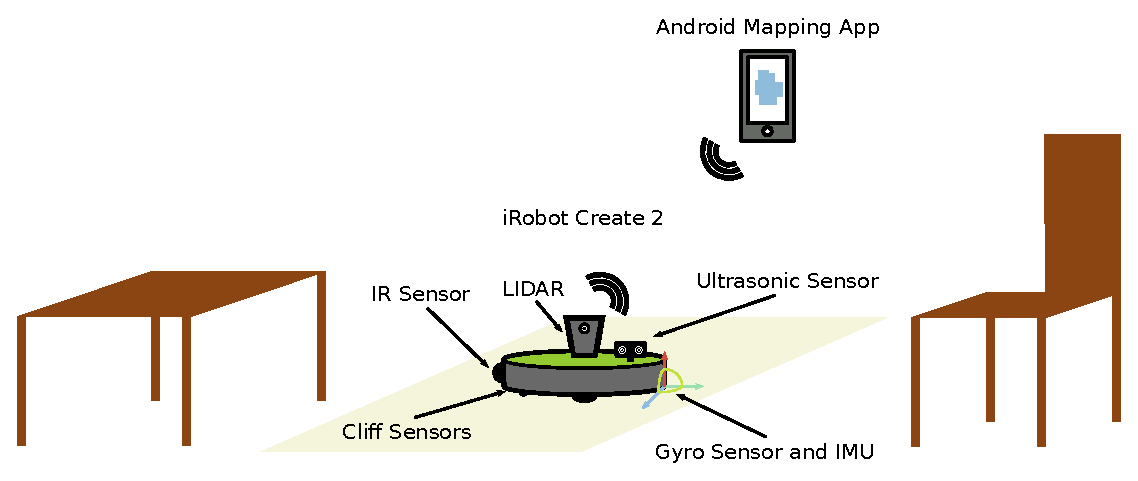
\includegraphics[scale=0.45]{figs/inkscape/mappingRobotArchitecture.eps}
    \caption{Diagram representing the working principle of the cleaning and mapping robot}
    \label{fig:my_label}
\end{figure}
\end{frame}

\section{Progress}

\begin{frame}{Progress}{}
    \begin{itemize}
        \item Created basic layout of the Android app for displaying the 2D room map in Android Studio
        \item Researched RPILidar S1 $360^\circ$ Laser Scanner
    \end{itemize}
\end{frame}

\begin{frame}{Progress}{}
    \begin{figure}
        \centering
        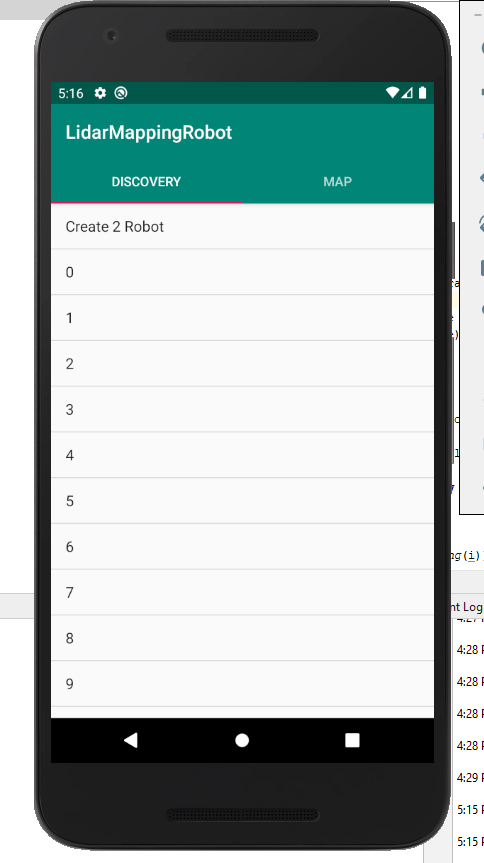
\includegraphics[scale=0.3]{figs/img/screenshot1}
        \caption{Screenshot of app with Discovery and Map tabs}
        \label{fig:my_label}
    \end{figure}
\end{frame}

\subsection{Further app details}
\begin{frame}{Progress}{Further app details}
    \begin{itemize}
        \item \texttt{TabLayout} View used for displaying tabs horizontally
        \item \texttt{Fragment} class used for both the discovery and map tabs
        \item To display items in a list, \texttt{ListView} is used for displaying a vertically-scrollable collection of views
        \item \texttt{ArrayAdapter} used for displaying Strings from an \texttt{ArrayList} in the \texttt{ListView}
        \item \texttt{AdapterView.setOnItemClickListener()} to register a callback when an item in the adapter view has been clicked
    \end{itemize}
\end{frame}

\subsection{Lidar}
\begin{frame}{Progress}{Lidar}
    \begin{figure}
        \centering
        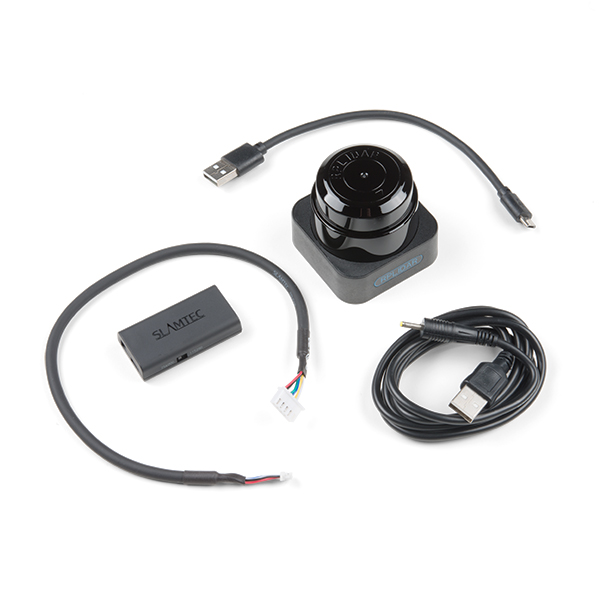
\includegraphics[scale=1]{figs/img/15872-Slamtec_RPLIDAR_S1-01.jpg}
        \caption{RPILidar S1 $360^\circ$ TOF Laser Scanner, source: https://www.sparkfun.com/products/15872}
        \label{fig:my_label}
    \end{figure}
\end{frame}

\begin{frame}{Progress}{Lidar}
    \begin{itemize}
        \item Takes samples at a rate up to 9200 samples per second
        \item 40 meter range
        \item Built-in motor that rotates at 10 Hz (600 rpm)
        \item Data is transferred over serial connection 256000 bps
        \item Can be connected to a single board computer (Beaglebone Blue)
        \item Separate power interfaces for the scanner and motor (5V VCC)
    \end{itemize}
\end{frame}

\section{Plans}
\begin{frame}{Plans}{}
    \begin{itemize}
        \item Build custom adapter class for displaying network data of the discovered robot
        \item Write a server in Python for the Beaglebone to accept connections from mobile devices
        \item In the \texttt{DiscoveryFragment} class add code to automatically start discovering robots with TCP/IP client code
        \item Add a spinner in the UI while the app is waiting for robot connections
    \end{itemize}
\end{frame}
% You can reveal the parts of a slide one at a time
% with the \pause command:
%\begin{frame}{Second Slide Title}
%  \begin{itemize}
%  \item {
%    First item.
%    \pause % The slide will pause after showing the first item
%  }
  %\item {   
  %  Second item.
 % }
  % You can also specify when the content should appear
  % by using <n->:
 % \item<3-> {
 %   Third item.
 % }
%  \item<4-> {
%    Fourth item.
 % }
  % or you can use the \uncover command to reveal general
  % content (not just \items):
%  \item<5-> {
%    Fifth item. \uncover<6->{Extra text in the fifth item.}
%  }
%  \end{itemize}
%\end{frame}

%\section{Second Main Section}

%\subsection{Another Subsection}

%\begin{frame}{Blocks}
%\begin{block}{Block Title}
%You can also highlight sections of your %presentation in a block, with it's own %title
%\end{block}
%\begin{theorem}
%There are separate environments for %theorems, examples, definitions and proofs.
%\end{theorem}
%\begin{example}
%Here is an example of an example block.
%\end{example}
%\end{frame}

% Placing a * after \section means it will not show in the
% outline or table of contents.
% \section*{Summary}

% \begin{frame}{Summary}
%   \begin{itemize}
%   \item
%     The \alert{first main message} of your talk in one or two lines.
%   \item
%     The \alert{second main message} of your talk in one or two lines.
%   \item
%     Perhaps a \alert{third message}, but not more than that.
%   \end{itemize}
  
%   \begin{itemize}
%   \item
%     Outlook
%     \begin{itemize}
%     \item
%       Something you haven't solved.
%     \item
%       Something else you haven't solved.
%     \end{itemize}
%   \end{itemize}
% \end{frame}



% All of the following is optional and typically not needed. 
\appendix
\section<presentation>*{\appendixname}
\subsection<presentation>*{For Further Reading}

\begin{frame}[allowframebreaks]
  \frametitle<presentation>{References}
    
  \begin{thebibliography}{10}
    
  \setbeamertemplate{bibliography item}[online]
  
  \bibitem{android}
  Android Developer Docs
  \newblock \url{https://developer.android.com/}
  
  \bibitem{lidardatasheet}
  RPILidar S1 360 Datasheet
  \newblock \url{https://www.robotshop.com/media/files/content/r/rpk/pdf/rplidar-s1-360-laser-scanner-40-m-datasheet.pdf}
  \end{thebibliography}
\end{frame}

\end{document}



%%% Local Variables:
%%% mode: latex
%%% TeX-master: t
%%% End:
